\entry{Semana del 30/06/2025}
\section{Transformada de Hilbert.}
Mientras intentaba pensar una forma de calcular la frecuencia instantánea para evitar los artefactos de la poca resolución en Fourier al graficar en tiempo real con ventana muy chiquitas ChatGPT sugirió calcular la función analítica:

\begin{equation}
	z(t)=x(t)+i\mathcal{H}\{x\}(t)=A(t)e^{i\phi(t)}
\end{equation} 

Donde $\mathcal{H}$ denota la transformada de Hilbert. Luego la frecuencia instantánea sería:

\begin{equation}
	\omega(t)=\frac{d\phi}{dt}
\end{equation}

Lo cual pareció funcionar bastante bien incluso cuando había pocos puntos (8192 a 500 kHz). 

Sin embargo, mientras trataba de entender qué era exactamente lo que hacía la función \textit{scipy.signal.hilbert} caí en que la Transformada de Hilbert lo que hace para obtener la función analítica es aplicar un desfasaje de $\pm\pi/2$ según si la frecuencia es mayor o menor a 0, al multiplicar por $i$ la FFT y luego hacer la IFFT. 

Entonces surgieron un par de ideas:
\begin{itemize}
	\item Usar la parte imaginaria de la función Hilbert de Scipy para obtener la cuadratura a partir de la señal de referencia, sin necesidad de calcular la frecuencia de la señal y la cantidad de puntos a retrasarla en función de ésta.
	\item Calcular directamente la fase instantánea de la señal de interés y de la referencia con la función analítica y obtener la fase relativa como la resta de ambas. Acá vamos a restar el término $\omega t$ de ambas así que es importante que efectivamente sea el mismo. Además como va a ser la fase instantánea va a ver que aplicarle un filtro pasabajos a posteriori para eliminar el ruido de frecuenicas altas.
\end{itemize}

\begin{figure}[th!]
	\centering
	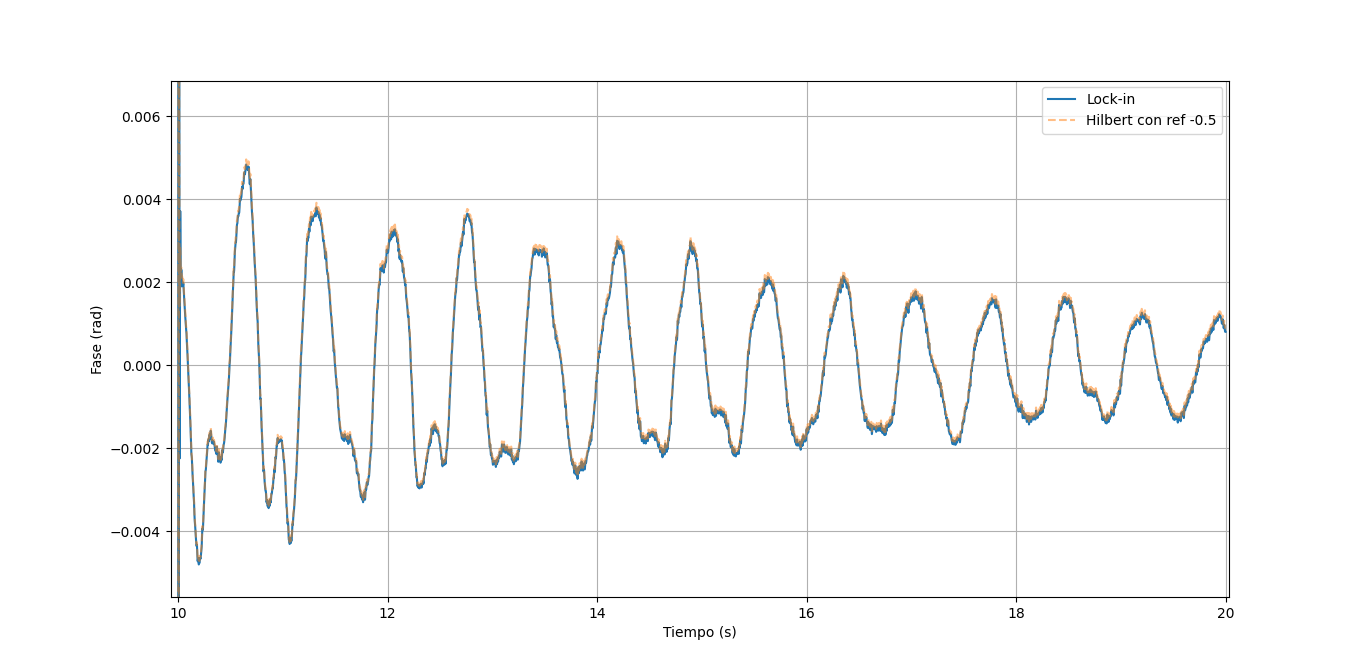
\includegraphics[width=0.87\linewidth]{Figures/30_06_2025/Hilbert_como_lock_in}
	\caption{Comparación del lock-in que veníamos usando y de la resta entre las fases instantáneas de la de señal de interés con fase modulada y su referencia, luego de pasarles un pasabajos, con $f_c=100$ Hz. Dan exactamente lo mismo, incluso el ruido es lo mismo para frecuencias de corte más altas. Lo único que cambia es el punto medio pero no nos interesa tanto, acá resté la media a ambas.} % k 
	\label{fig:hilbertcomolockin}
\end{figure}
